\documentclass[]{article}
\usepackage{amsmath}
\usepackage{graphicx}
%opening
\title{}
\author{}
\usepackage[utf8]{inputenc} 

\begin{document}

%\maketitle

%\begin{abstract}
%\end{abstract}
\section{Time evolution of coarse states on static interaction networks with different topologies}
\subsection{Fully connected network}

Figure \ref{fig:time_evolution} shows the ensemble average over 250 realizations of the average state in a fully connected network as a function of time. Simulations are performed for two different coupling constants $\mathcal{N}(\bar{\nu}=0.5)$ and  $\mathcal{N}(\bar{\nu}=0.05)$ and two different initial conditions $ \mu_{0 n} \sim \mathcal{B} ( \mu; 0.5) $ respectively $ \mu_{0n} \sim\mathcal{B} ( \mu; 0.9 ) $ for $n=1,...,500$.     %\ref{} . 
 The values of the microscopic parameters are chosen in correspondence with these in the AHS-lattice-model \cite{avitabile14}. Each agent is interacting with all other agents. For small values of the average coupling constant $\bar{\nu}$, the mixed state is the unique macroscopic stable equilibrium.  If the average value of the coupling constant $\bar{\nu}$ is increased, two new macroscopic states arise, suggesting the presence of a pitchfork bifurcation. 

%For a network with 8000 nodes with all-to-all-coupling (all agents in the network interact with all the other agents).
\subsection{Erd\H{o}s-Rényi network}

Above described experiments are repeated with the same simulation parameters and system size, but with all agents randomly connected with on average 10 other agents. The connections don't change in time and the agents only interact with agents they are connected with. Figure \ref{fig:time_evolution_erdos} shows that it took at least 20 iterations to achieve the locked-in states, which is longer than the time needed to reach equilibrium in a fully connected network. For the mixed state however, the relaxation time does not differ significantly between both models.

\subsection{Small world network}

The simulations are repeated for a small world network, generated by the Watts-Strogatz-algorithm with rewiring probability $\beta=0.5$. This accounts for higher clustering in comparison with the Erd\H{o}s-Rényi-network, while each agent still stays connected with on average 10 other agents. Figure \ref{fig:time_evolution_watts} shows that the time to achieve the locked-in-states lies between the time on a fully-connected-network and the time on an Erd\H{o}s-Rényi-network with same system size. 


\begin{figure}


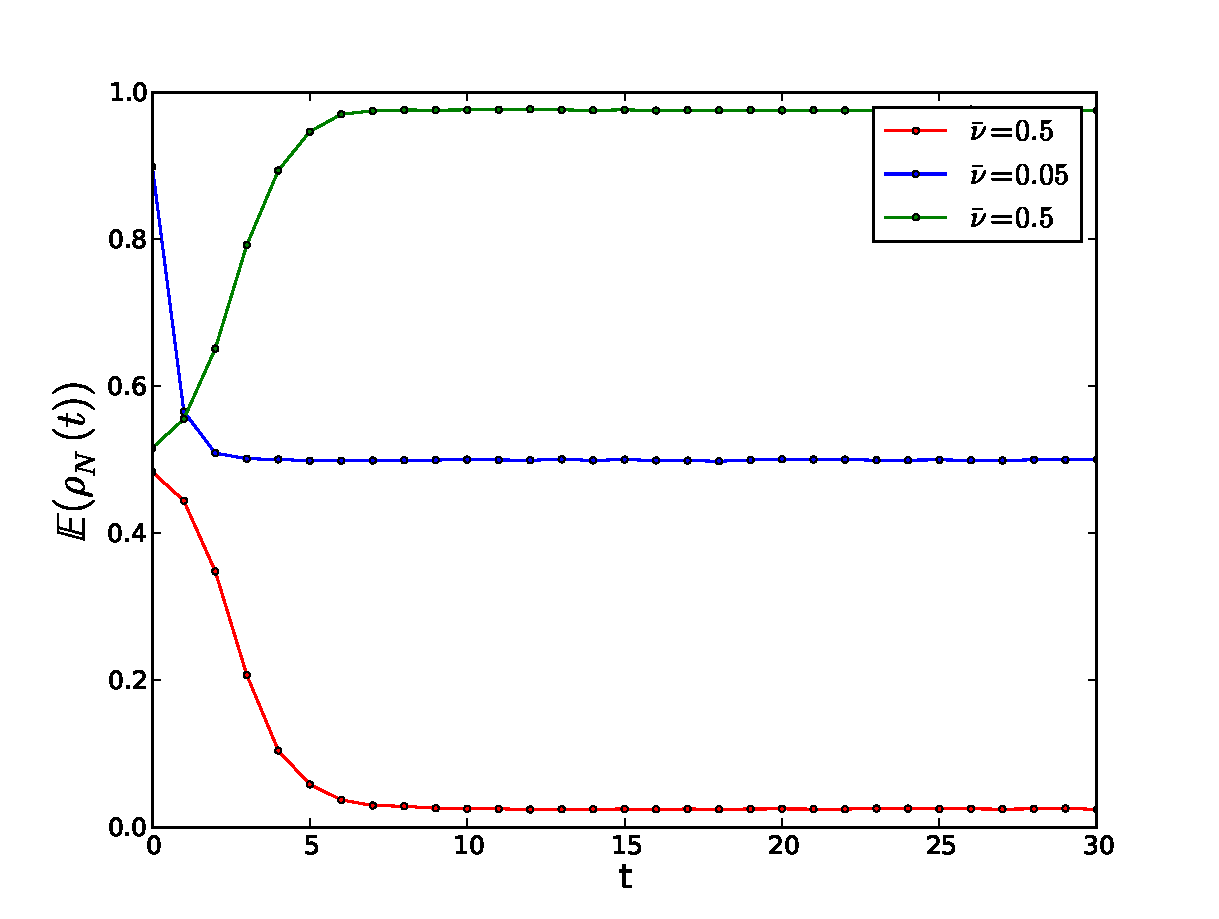
\includegraphics[width=0.9\textwidth]{time_evolution_M250_N500.pdf}
\caption{Average time evolution of coarse states in a fully-connected network with 500 nodes.}
\label{fig:time_evolution}
\end{figure}


\begin{figure}
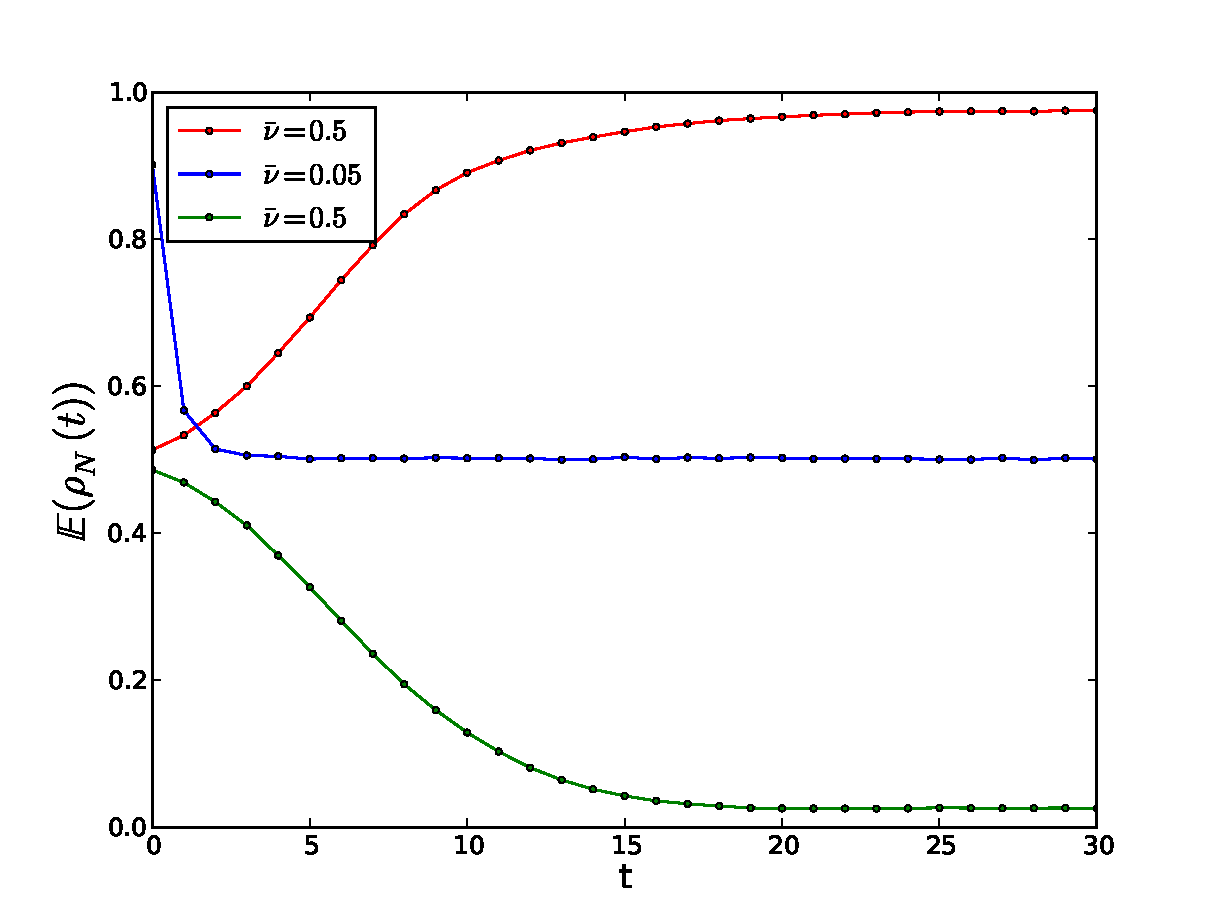
\includegraphics[width=0.9\textwidth]{time_evolution_erdos10_M250_N500.pdf}
\caption{Average time evolution of coarse states in an Erd\H{o}s-Rényi network of 500 nodes with average degree 10.}
\label{fig:time_evolution_erdos}
\end{figure}


\begin{figure}
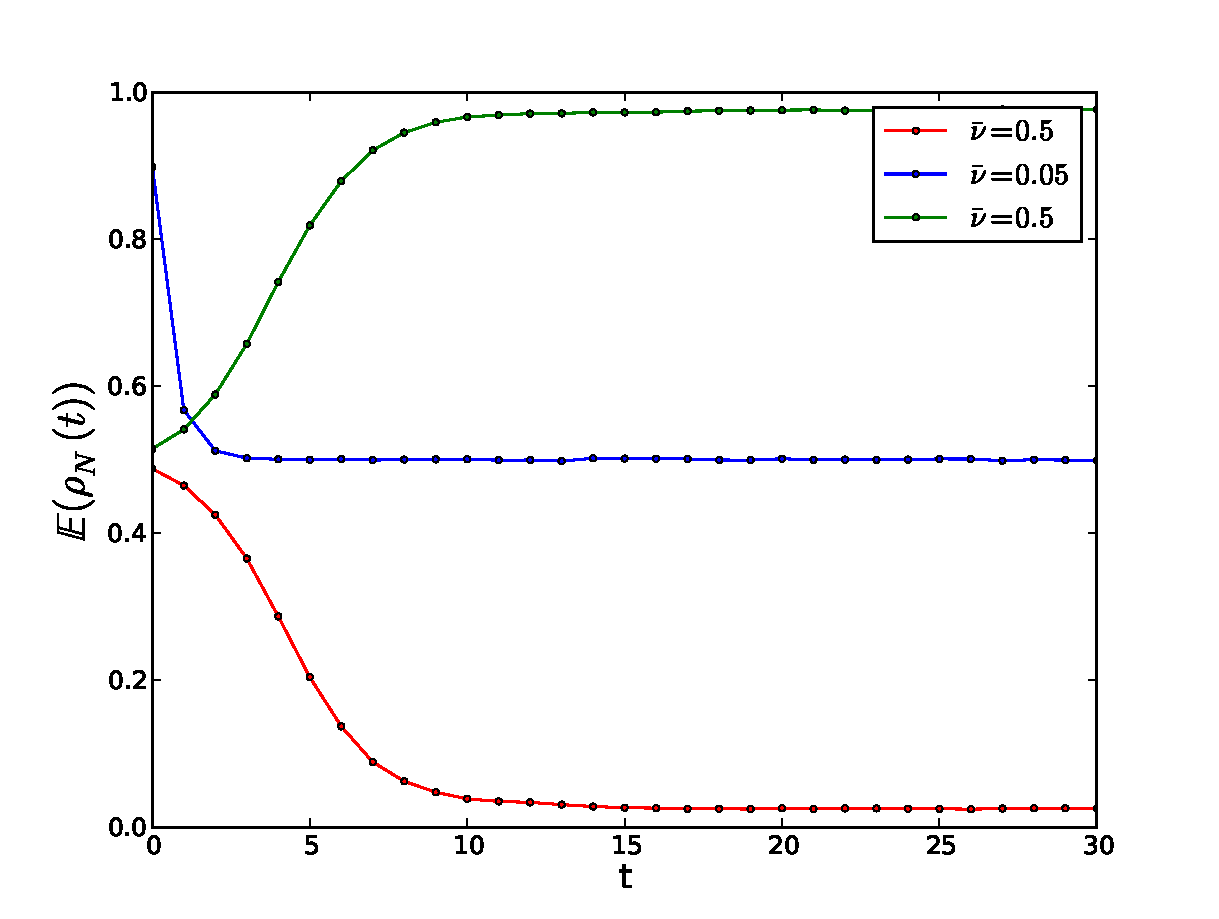
\includegraphics[width=0.9\textwidth]{time_evolution_small_world_beta5_M250_N500.pdf}
\caption{Average time evolution of coarse states in a Watts-Strogatz network ($\beta=0.5$) with  500 nodes and average degree 10.}
\label{fig:time_evolution_watts}
\end{figure}






\bibliographystyle{plain}
\bibliography{biblio.bib}
\end{document}



